
\begin{question}
Consider the following time series on Australian wine sales:

\begin{figure}[H]
\centering
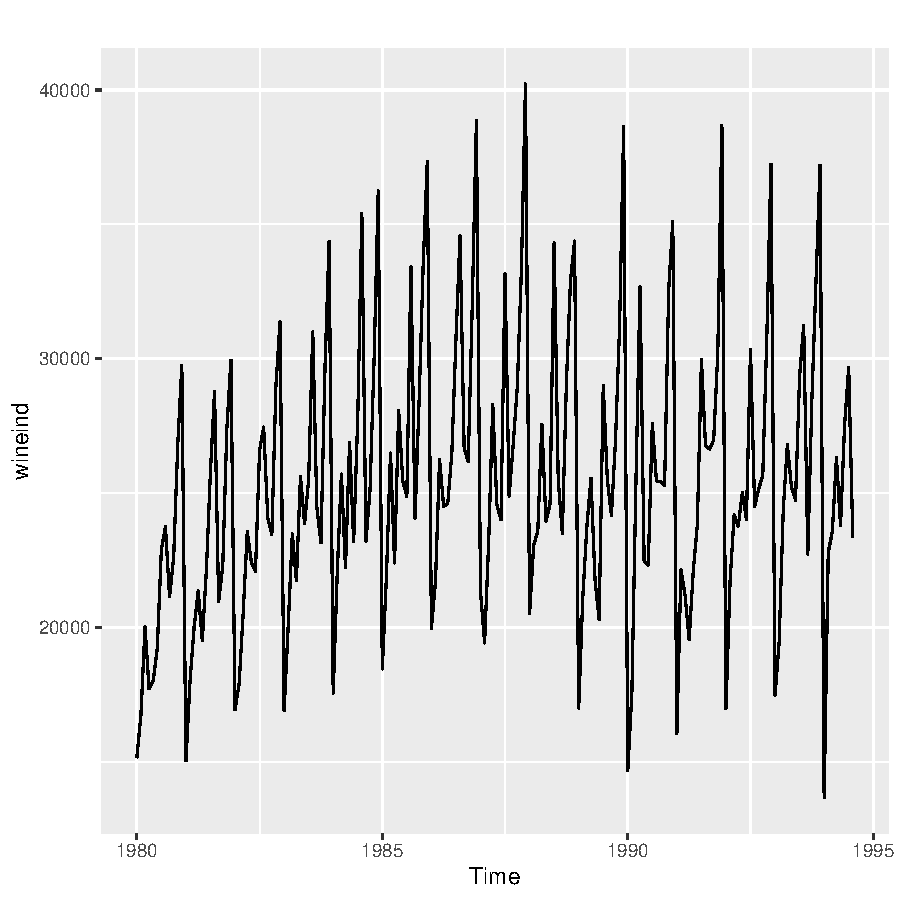
\includegraphics{unnamed-chunk-1-1-3.pdf}
\caption{plot of chunk unnamed-chunk-1}
\end{figure}

Which parameter for Box-Cox transformation can be used for this time series to deal with growing amplitude of seasonality?
\begin{answerlist}
  \item \(\lambda=1\) You can load the gas wineind in R by importing forecast library or if you use other programming languages you can download it \href{https://github.com/vincentarelbundock/Rdatasets/blob/master/csv/forecast/wineind.csv}{here}.
  \item \(\lambda=0\)
  \item \(\lambda=-2\)
  \item \(\lambda=0.5\)
\end{answerlist}
\end{question}

\begin{solution}
\begin{answerlist}
  \item False. Oscillations amplitude grows over time
  \item True.
  \item False. Oscillations are unstable
  \item True.
\end{answerlist}
\end{solution}

